% MIT License

% Copyright (c) 2022 Chiyuru

% Permission is hereby granted, free of charge, to any person obtaining a copy of this software and associated documentation files (the "Software"), 
% to deal in the Software without restriction, including without limitation the rights
% to use, copy, modify, merge, publish, distribute, sublicense, and/or sell
% copies of the Software, and to permit persons to whom the Software is
% furnished to do so, subject to the following conditions:

% The above copyright notice and this permission notice shall be included in all copies or substantial portions of the Software.

% THE SOFTWARE IS PROVIDED "AS IS", WITHOUT WARRANTY OF ANY KIND, EXPRESS OR IMPLIED, INCLUDING BUT NOT LIMITED TO THE WARRANTIES OF MERCHANTABILITY,
% FITNESS FOR A PARTICULAR PURPOSE AND NONINFRINGEMENT. IN NO EVENT SHALL THE AUTHORS OR COPYRIGHT HOLDERS BE LIABLE FOR ANY CLAIM, DAMAGES OR OTHER
% LIABILITY, WHETHER IN AN ACTION OF CONTRACT, TORT OR OTHERWISE, ARISING FROM,
% OUT OF OR IN CONNECTION WITH THE SOFTWARE OR THE USE OR OTHER DEALINGS IN THE SOFTWARE.

\documentclass[UTF8]{ctexart}

\usepackage{amssymb}
\usepackage{amsmath}
\usepackage{cases}
\usepackage{cite}
\usepackage{graphicx}
\usepackage{subfigure}
\usepackage[margin=1in]{geometry}
\geometry{a4paper}
\usepackage{fancyhdr}
\pagestyle{fancy}
\fancyhf{}


\title{基于人工智能的量化交易设计报告}
\author{
    刘锦坤
    \\2022013352}
\date{\today}
\pagenumbering{arabic}

\begin{document}

\fancyhead[C]{基于人工智能的量化交易设计报告}
\fancyfoot[C]{\thepage}

\maketitle
\begin{abstract}
    本项目旨在设计一个基于人工智能的量化交易策略。通过建立一个LSTM神经网络模型,根据过去一段时间内的股票交易数据,预测接下来一段时间内股票的涨跌情况,从而制定特定的交易策略,实现经济收益。我在项目中主要负责项目的整体设计,数据采集,数据预处理,模型设计,模型搭建和训练的代码实现,因此本报告将主要聚焦于这一部分。
\end{abstract}
\tableofcontents
\newpage

\section{项目背景}
在股票市场中,投资者常常将过去一段时间内的股票交易数据进行处理,从而得到为若干技术指标。常见的有移动平均线(MA)、指数平滑移动平均线(EMA)、布林带(Bollinger Bands)、平滑异同移动平均线(MACD)等。投资者会根据这些指标的变化形态,制定特定的交易策略,以获得更好的投资收益。根据特定的策略进行交易,这即是量化交易的基本思想。

但是根据传统的技术指标交易存在明显的不足。首先,这些技术交易指标的计算全部依赖利用某一种显式的计算方法进行计算的,这样的显式的计算方法本身很有可能并不能捕捉到股票市场全部的交易规律。其次,股票市场是典型的二级响应系统,即市场上的交易行为会对市场本身产生影响,而这种影响又会反过来影响交易行为。这就导致任何一种依靠传统技术指标的交易策略,尤其是被大量投资者采用的交易策略,都会面临市场反作用导致的失效性的问题。

而人工智能技术的发展,尤其是神经网络模型的发展,为量化交易提供了新的思路。神经网络通过隐式的表达方法,能够对股票交易市场中大批量的过往交易数据进行学习,从而捕捉到更全面的交易规律。同时由于这样的交易策略并不显式的依赖于任何传统的技术指标,因此更有可能避免传统技术指标交易策略的失效性问题。基于这种想法,本项目将尝试设计一个基于人工智能的量化交易策略。

\section{项目设计}
\subsection{基本目标}
最终制定的项目基本目标为:根据过去一段时间内(days\_before)一支股票的交易数据,判断接下来一段时间(days\_after)内,股票呈现多头趋势还是空头趋势(股价是上涨还是下跌),根据模型的判断买入和卖出股票,实现经济收益。
\subsection{模型方案}
而施行该目标的基本方案为:建立一个LSTM神经网络模型,模型输入为过去一段时间的交易数据,预期输出接下来一段时间内股票上涨和下跌的概率。

\section{数据采集}
由于我们的基本实现方案是利用神经网络模型从过往的交易数据中学习特征,从而应用于未来的交易预测,这就需要大量的过往交易数据。在数据获取和整理上,我们外联了聚宽量化投研平台(JoinQuant平台),由聚宽为我们提供过往股票交易数据。可以通过其提供的Python的API访问获取过往股票交易数据。用于下一步的数据处理。
\begin{figure}[htbp]
    \centering
    
\includegraphics[height = 3cm]{./images/JoinQuant.PNG}
    \caption{JoinQuant平台}
    \label{fig:JQ}
\end{figure}

\section{模型选择}
\subsection{RNN\&LSTM模型}
股票数据属于典型的时间序列数据,查阅相关资料发现,RNN(Recurrent Neural Network)类神经网络如图\ref{fig:RNN}以其独特的构造适合时间序列的模型。
\begin{figure}[h]
    \centering
    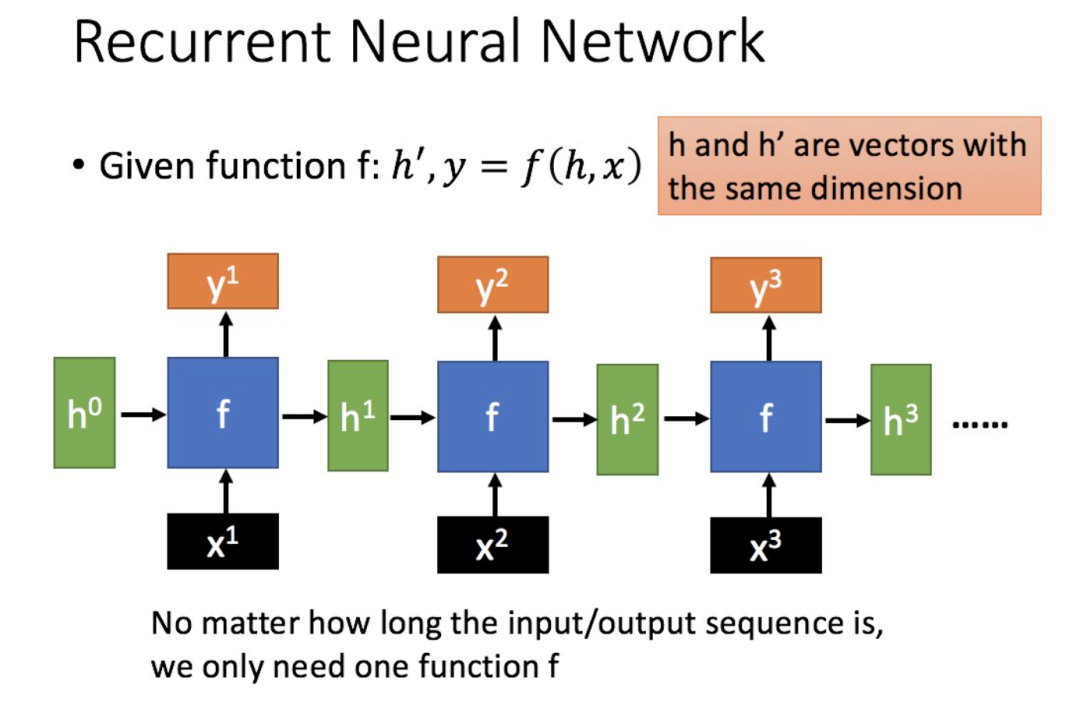
\includegraphics[width=0.7\textwidth]{images/RNN.png}
    \caption{RNN模型示意图}
    \label{fig:RNN}
\end{figure}

但是RNN模型存在对于长距离关系捕捉的不足,序列前端的信息可能在循环传递中被遗忘,对于股票来说,以前的一次暴跌和暴涨很可能就会影响后续投资者的信心,因此我们最终采取了LSTM(Long Short Term Memory)网络如图\ref{fig:LSTM}。
\begin{figure}[h]
    \centering
    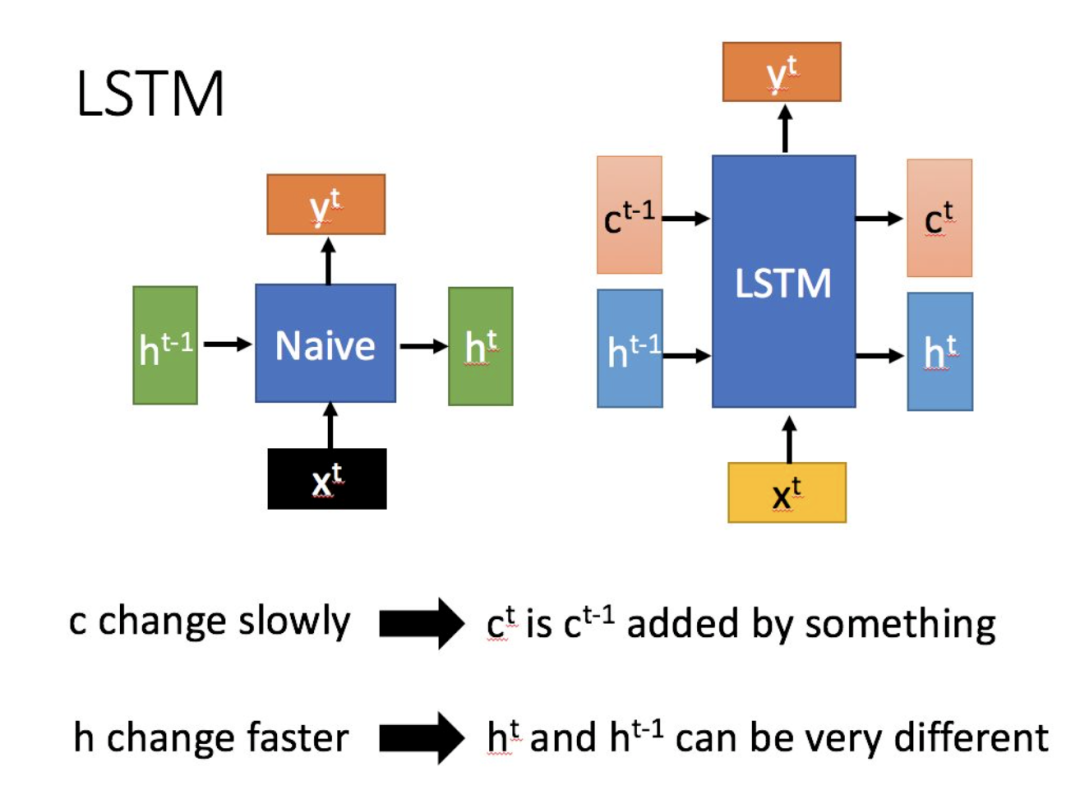
\includegraphics[width=0.7\textwidth]{images/LSTM.png}
    \caption{LSTM模型示意图}
    \label{fig:LSTM}
\end{figure}
\subsection{最终模型}
最终,设计模型架构如图\ref{fig:Model}所示。输入数据先直接输入到LSTM网络中,取LSTM层最后一个神经元的输出,然后通过全连接层经过逻辑回归(SoftMax)输出预测结果(涨跌概率)。
\begin{figure}[htbp]
    \centering
    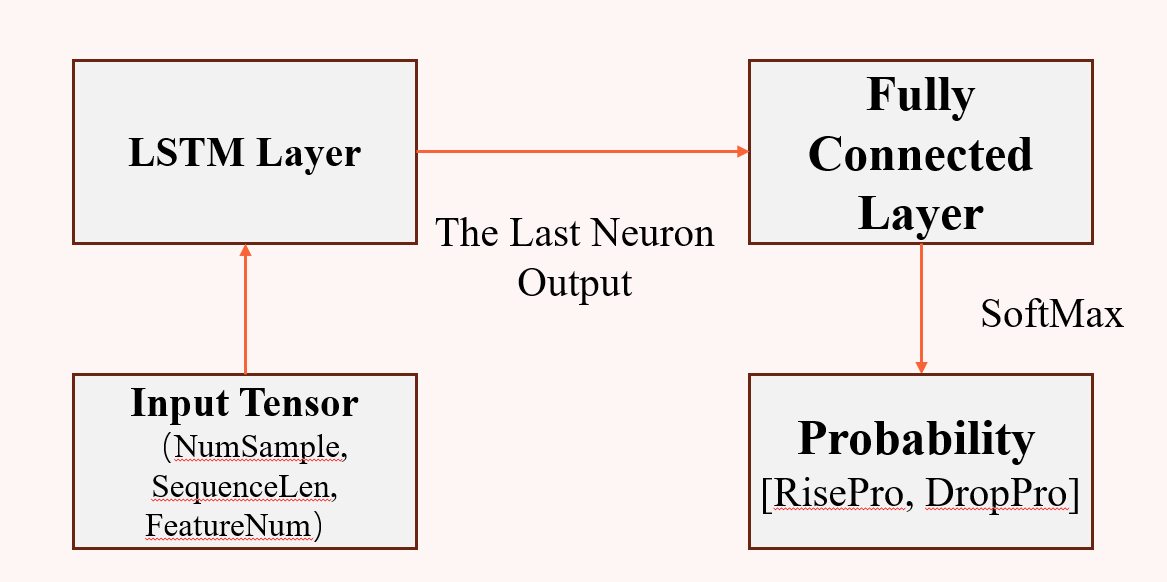
\includegraphics[width=0.8\textwidth]{images/model.png}
    \caption{模型架构}
    \label{fig:Model}
\end{figure}
\section{数据预处理}
\subsection{原始数据}
根据聚宽提供的数据,最终汇集整理了目标股票在过去每天的开盘价、收盘价、盘中高价、盘中低价、成交量、成交额、前一天收盘价、成交均价八大数据作为原始特征数据。
\subsection{量比处理}
对于神经网络模型的训练,好的数据预处理可以使得神经网络模型更好的发掘数据中的特征,在数据预处理阶段,我们对数据进行了如下量比处理:

借鉴股票交易市场投资者常讨论的几个技术形态,(例如放量上涨,缩量上升),并且考虑到中国a股市场的特性,认为股票量、价的绝对值并不具有参考意义,而是采用了量比方案进行数据处理,即对于上述八大原始数据,我们以每一天的原始数据和前一天的比值作为输入特征。
\subsection{数据标准化}
神经网络模型对数据的尺度敏感,因此我们对输入数据最后进行了标准化处理,即对于每一个特征,我们将其利用MinMax标准化方法,将其缩放到[0,1]之间。
\subsection{数据集划分}
为了使得回测有意义,我们严格的将训练集和测试集按照时间先后分开,仅在训练集上进行训练,最后在测试集上进行收益回测,保证不发生数据的泄露。

\section{部署和训练}
最终我们利用Pytorch框架搭建了上述模型训练,相关细节如下:
\begin{itemize}
    \item 由于问题本身接近分类问题(看涨或看跌),所以采用了CrossEntropyLoss(交错熵)作为损失函数。
    \item 采用Adam优化器进行模型参数的优化。
    \item 为了克服过拟合现象,采取了dropout手段,在训练时会随机丢弃部分神经元。
    \item 为了加速训练,使用了本地的RTX3060和RTX4060,利用CUDA进行了GPU加速计算。
    \item 为了获得更好的回测效果,我们进行了大量超参数的调节,包括days\_before, days\_after, batch\_size(训练批次大小), hidden\_size(LSTM网络隐藏层个数), num\_layer(LSTM网络的堆叠层数), dropout(训练时的丢弃概率)等。
\end{itemize}

\section{回测收益}
这一部分,我们以股票代码为002765.XSHE的蓝黛科技股票为例,适当调节超参数,在训练集上训练模型,再根据模型制定特定的交易策略后,在测试集上进行了回测。
\subsection{交易策略}
制定的交易策略如图\ref{fig:strategy}所示。
\begin{itemize}
    \item 当模型预测的上涨概率大于$P_b$时以收盘价买入。
    \item 买入后若模型预测上涨概率小于$P_s$卖出,或跌幅大于20\%止损。    
\end{itemize}
\begin{figure}[htbp]
    \centering
    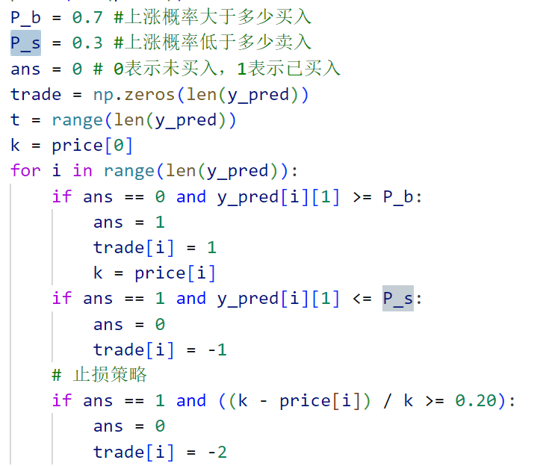
\includegraphics[width=0.5\textwidth]{images/strategy.png}
    \caption{交易策略}
    \label{fig:strategy}
\end{figure}
\subsection{收益结果}
最终利用制定的策略,在测试集上回测,收益效果如图\ref{fig:profit}所示。
\begin{figure}[htbp]
    \centering
    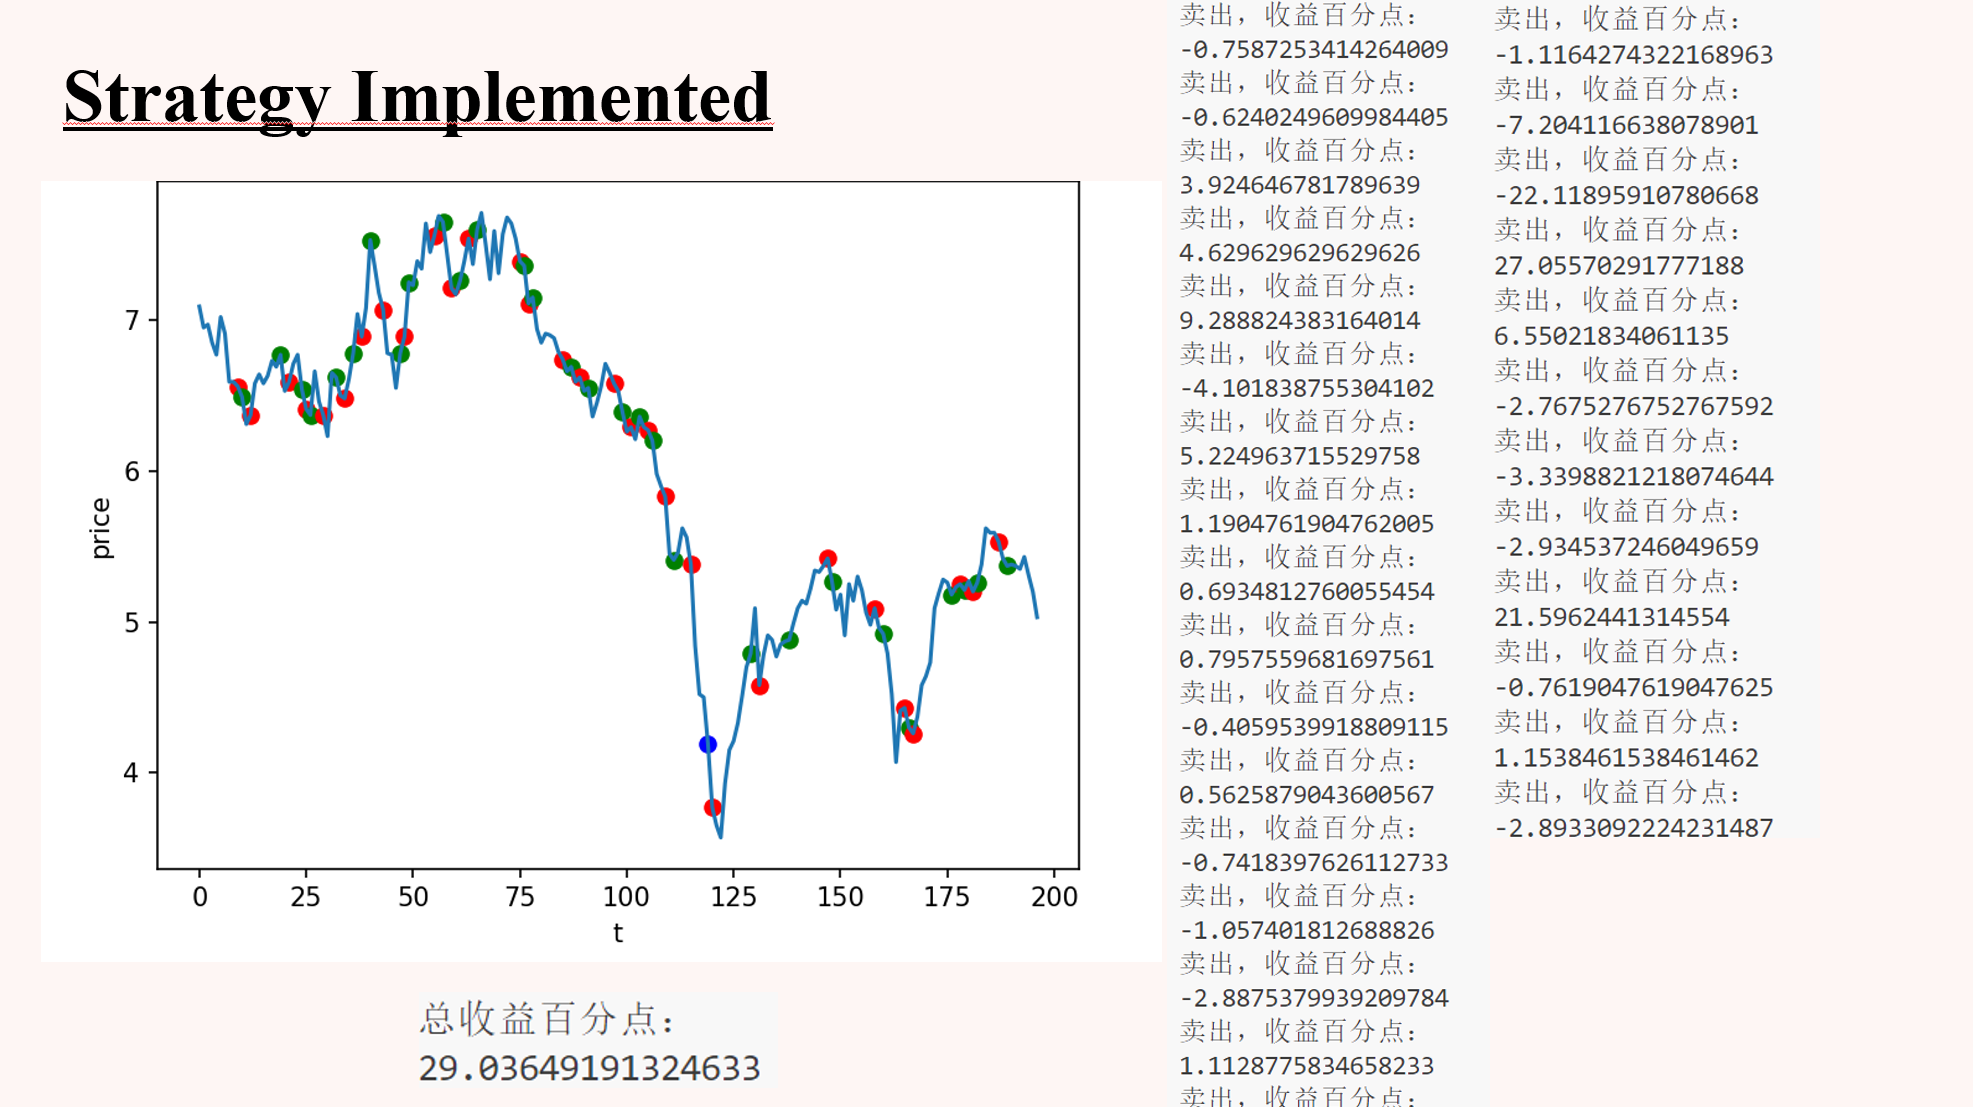
\includegraphics[width=0.9\textwidth]{images/profit.png}
    \caption{收益曲线}
    \label{fig:profit}
\end{figure}
其中红色的点代表买入点,而绿色的点代表卖出点,蓝色的点代表止损卖出点,最后可以看到,在测试集约200个交易日中,在这样一支整体下行的股票上,我们的策略实现了约29\%的盈利,这表明我们的策略确实是有效的。
\section{分工}
项目的整体分工如下:
\begin{itemize}
    \item 刘锦坤:负责项目的整体设计,数据采集,数据预处理,模型设计,模型搭建和训练的代码实现。
    \item 郭锐冰:负责模型超参数的调节,交易策略的制定,回测收益的计算。
    \item 陈飞扬:负责最终展示PPT的美化设计。
\end{itemize}
\end{document}
